% !TeX root = ..\main.tex
\pagestyle{fancy-style}
\npchapter{Einleitung}
\pagenumbering{arabic}

\section{Motivation}
Die kontinuierliche Evolution von Softwaretechnologien und -umgebungen hat einen erheblichen Einfluss auf die Entwicklung und Leistung von Anwendungen. Kürzlich wurde die Version 1.0 der JavaScript Laufzeitumgebung Bun veröffentlicht, die vielversprechende Verbesserungen in Bezug auf die Leistung im Vergleich zu Node.js ankündigt \cite{Sumner.2023}. \newline
JavaScript ist eine Programmiersprache, die vor allem im Kontext der Web-Entwicklung verwendet wird \cite{Brown.November2019}. Aktuell erfreut sich JavaScript großer Beliebtheit. In einer Umfrage an Entwickler von Stack Overflow wurden mehr als 89.000 Entwickler befragt. JavaScript ist zum 11. Jahr in Folge die am häufigsten verwendete Programmiersprache. Mehr als 63\% der befragten Entwickler haben JavaScript als beliebteste Technologie gewählt. Bei den professionellen Entwicklern ist der Anteil mit mehr als 65\% sogar noch höher. Außerdem ist TypeScript, eine stark typisierte Programmiersprache, die auf 
JavaScript aufbaut, unter den Teilnehmer auch beliebt. Ca. 39\% aller Entwickler und ca. 44\% der professionellen Entwickler verwenden auch TypeScript. Damit ist TypeScript die 4. beliebteste Programmiersprache. \cite{StackOverflow.2023} Daraus folgt, dass das Ökosystem von JavaScript eine hohe Praxisrelevanz besitzt. \\

\begin{figure}[h]
	\centering
	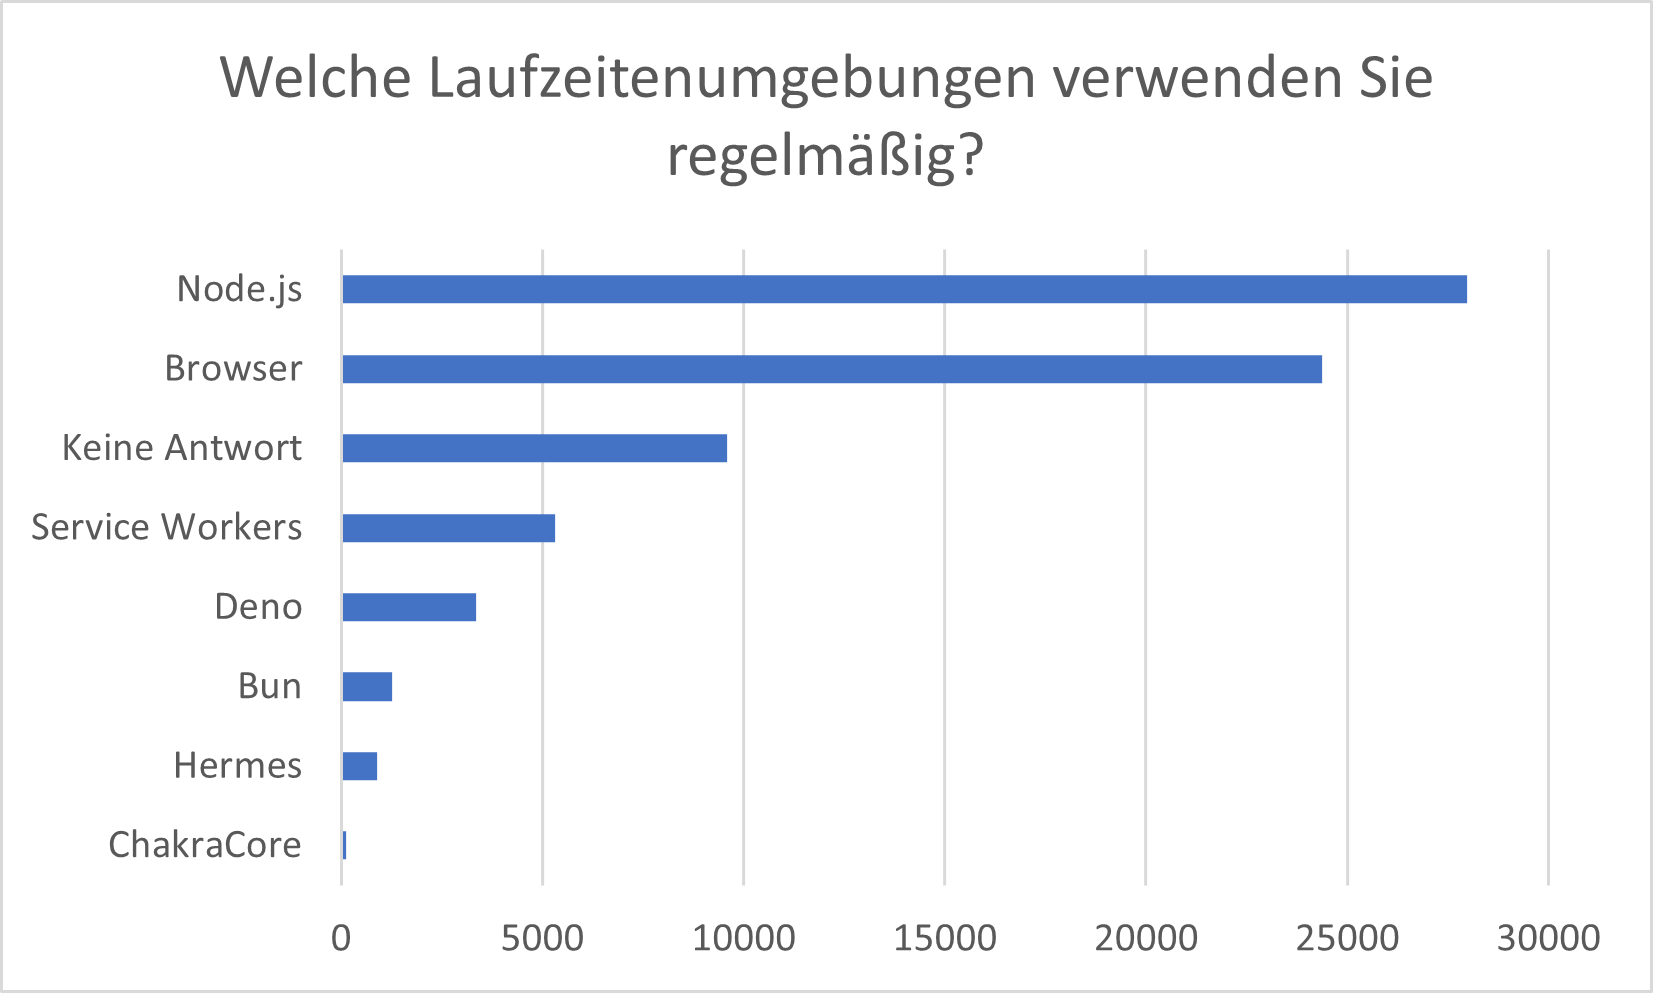
\includegraphics[width=\linewidth]{./images/WhichRuntimesDoYouUseRegularly}
	\caption{Nutzungsstatistik von JavaScript-Laufzeitumgebungen \cite{Greif.2022}}
	\label{fig:runtime-share}
\end{figure}

\noindent
JavaScript wird nicht nur für die Entwicklung im Frontend, sondern auch für die Entwicklung im Backend 
verwendet, ungefähr 3\% der weltweit bekannten Server verwenden eine Laufzeitumgebung, die JavaScript 
ausführen kann. \cite{QSuccess.2023} Um JavaScript auf einem Server ausführen zu können, wird eine Laufzeitumgebung benötigt. Wie Abbildung \ref{fig:runtime-share} zeigt, ist Node.js die am weitesten verbreitete Laufzeitumgebung. In der gezeigten Umfrage zum Zustand von JavaScript beantworteten ca. 71\% von 30.000 befragten Entwickler, dass sie Node.js als Laufzeitumgebung regelmäßig verwenden.
Nur ca. 9\% der befragten Entwickler verwenden Deno und ca. 3\% Bun als eine Alternative zu Node.js. \cite{Greif.2022}


\section{Zielsetzung}
Aktuell ist Node.js die Laufzeitumgebung, die am weitesten verbreitet ist. Dennoch gibt erscheinen immer wieder neue Laufzeitumgebungen für JavaScript, die versuchen Node.js zu verdrängen. Eine mögliche Alternative ist Bun, das am 9. September 2023 in der Version 1.0 veröffentlicht worden ist. Die Entwickler von Bun werben mit Features wie erheblicher Performancesteigerung, eleganten Schnittstellen und einer angenehmen Entwicklererfahrung. \cite{Sumner.2023} \\

\noindent
Das Hauptziel dieser Arbeit besteht darin, die Version 1.0 der JavaScript Laufzeitumgebung Bun einer eingehenden Evaluierung zu unterziehen. Konkret wird untersucht, ob die in den Ankündigungen versprochene signifikante Leistungssteigerung im Vergleich zu Node.js tatsächlich existiert und reproduzierbar ist. Darüber hinaus wird geprüft, inwiefern bestehende Projekte auf der Basis von Node.js mit Bun kompatibel sind. Die Ergebnisse dieser Arbeit können Entwicklern bei der Entscheidung helfen, ob sie auf Bun 1.0 migrieren sollten, und sie dabei unterstützen, die Leistung ihrer bestehenden Projekte zu verbessern. Insgesamt zielt diese Untersuchung darauf ab, Klarheit über die Versprechungen von Bun 1.0 zu schaffen und Entwicklern fundierte Informationen für ihre Entscheidungsfindung zur Verfügung zu stellen. Dies spiegelt sich in den folgenden Leitfragen wider:
\begin{itemize}
    \item Welche konkreten Leistungsverbesserungen können in Bun 1.0 im Vergleich zu Node.js festgestellt werden, und wie lassen sie sich quantifizieren?
    \item Inwiefern sind Projekte auf der Basis von Node.js kompatibel mit Bun? Wie schwierig gestaltet sich die Migration?
    \item Welche Herausforderungen und potenziellen Vorteile ergeben sich bei der Verwendung von Bun 1.0 im Vergleich zu Node.js für Entwickler und Projekte?
\end{itemize}

\section{Aufbau der Arbeit}
\todo{Kapitel schreiben}


